Ein Auto fährt an und fährt dann mit konstanter Geschwindigkeit weiter. Das Diagramm zeigt seine Geschwindigkeit.
\begin{center}
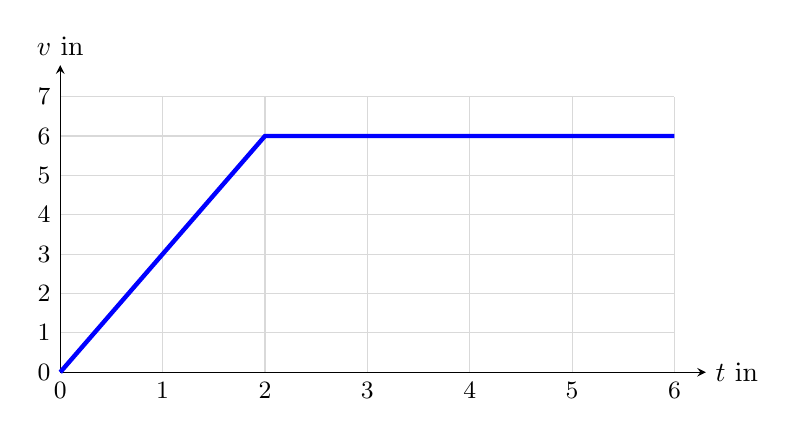
\begin{tikzpicture}[>=stealth, x=1.3cm, y=0.5cm]
 \draw[gray!30] (0,0) grid[xstep=1, ystep=1] (6,7);
 \draw[->] (0,0) -- (6.308,0) node[right] {$t$ in \si{\second}};
 \draw[->] (0,0) -- (0,7.8) node[above] {$v$ in \si{\meter\per\second}};
 \foreach \tk in {0,1,2,3,4,5,6} \node[below] at (\tk,0) {\small $\tk$};
 \foreach \yk in {0,1,2,3,4,5,6,7} \node[left] at (0,\yk) {\small $\yk$};
 \draw[ultra thick, blue] (0,0) -- (2,6) -- (6,6);
\end{tikzpicture}
\end{center}
\begin{abcliste}
\abc Bestimmen Sie die mittlere Geschwindigkeit von \SI{0}{\second} bis \tEO.
\abc Sara rechnet: „Am Anfang \SI{0}{\meter\per\second}, am Schluss \SI{6}{\meter\per\second}, im Mittel also \SI{3}{\meter\per\second}.“ Was ist an ihrer Rechnung falsch?
\end{abcliste}
